\documentclass{beamer}
\usepackage[utf8]{inputenc}

\usetheme{Madrid}
\usecolortheme{default}
\usepackage{amsmath,amssymb,amsfonts,amsthm}
\usepackage{txfonts}
\usepackage{tkz-euclide}
\usepackage{listings}
\usepackage{adjustbox}
\usepackage{array}
\usepackage{tabularx}
\usepackage{gvv}
\usepackage{lmodern}
\usepackage{circuitikz}
\usepackage{tikz}
\usepackage{graphicx}
\usepackage[T1]{fontenc}
\usepackage[utf8]{inputenc}

\lstset{
  language=Python,
  basicstyle=\ttfamily\small,
  breaklines=true,
  literate={λ}{{$\lambda$}}1
}



\setbeamertemplate{page number in head/foot}[totalframenumber]

\usepackage{tcolorbox}
\tcbuselibrary{minted,breakable,xparse,skins}



\definecolor{bg}{gray}{0.95}
\DeclareTCBListing{mintedbox}{O{}m!O{}}{%
  breakable=true,
  listing engine=minted,
  listing only,
  minted language=#2,
  minted style=default,
  minted options={%
    linenos,
    gobble=0,
    breaklines=true,
    breakafter=,,
    fontsize=\small,
    numbersep=8pt,
    #1},
  boxsep=0pt,
  left skip=0pt,
  right skip=0pt,
  left=25pt,
  right=0pt,
  top=3pt,
  bottom=3pt,
  arc=5pt,
  leftrule=0pt,
  rightrule=0pt,
  bottomrule=2pt,
  toprule=2pt,
  colback=bg,
  colframe=orange!70,
  enhanced,
  overlay={%
    \begin{tcbclipinterior}
    \fill[orange!20!white] (frame.south west) rectangle ([xshift=20pt]frame.north west);
    \end{tcbclipinterior}},
  #3,
}
\lstset{
    language=C,
    basicstyle=\ttfamily\small,
    keywordstyle=\color{blue},
    stringstyle=\color{orange},
    commentstyle=\color{green!60!black},
    numbers=left,
    numberstyle=\tiny\color{gray},
    breaklines=true,
    showstringspaces=false,
}
\begin{document}

\title 
{5.8.13}
\date{October 3,2025}


\author 
{Bhoomika V - EE25BTECH11015}




\frame{\titlepage}
\begin{frame}{Question}
\[
\text{Find the area of the triangle } ABC \text{ whose vertices are }\\ \\
\vec{A}(2,5),\; \vec{B}(4,7),\; \vec{C}(6,2).
\]
\end{frame}

\begin{frame}{equations}
Let the two numbers be $x$ and $y$ ($x > y$).

 Define equations
From the problem:

\[
x - y = 26
\]
\[
x = 3y
\]
\end{frame}

\begin{frame}{matrix form}
Rewriting in standard form $Ax = b$:

\[
\begin{cases}
x - y = 26 \\
x - 3y = 0
\end{cases}
\]


 Matrices $A$ and $b$

\[
A = 
\begin{bmatrix}
1 & -1 \\
1 & -3
\end{bmatrix}, 
\quad
b = 
\begin{bmatrix}
26 \\
0
\end{bmatrix}, 
\quad
\mathbf{x} = 
\begin{bmatrix}
x \\ y
\end{bmatrix}
\]
\end{frame}

\begin{frame}{using RREF}
So the system is:

\[
A \vec{x} = b
\]

 Reduce $A$ to RREF (only $A$)

Start with:

\[
A = 
\begin{bmatrix}
1 & -1 \\
1 & -3
\end{bmatrix}
\]

Eliminate first column in row 2

\[
R_2 \to R_2 - R_1 \implies 
\begin{bmatrix}
1 & -1 \\
0 & -2
\end{bmatrix}
\]


\end{frame}

\begin{frame}
\[
R_2 \to -\frac{1}{2} R_2 \implies 
\begin{bmatrix}
1 & -1 \\
0 & 1
\end{bmatrix}
\]



\[
R_1 \to R_1 + R_2 \implies 
\begin{bmatrix}
1 & 0 \\
0 & 1
\end{bmatrix}
\]

So the RREF of $A$ is the identity matrix:

\[
\text{RREF}(A) = I_2 = 
\begin{bmatrix}
1 & 0 \\
0 & 1
\end{bmatrix}
\]
\end{frame}

\begin{frame}
Solve $A \mathbf{x} = b$

Using the original $b$:

\[
\begin{bmatrix}
1 & 0 \\
0 & 1
\end{bmatrix}
\begin{bmatrix} x \\ y \end{bmatrix} =
\begin{bmatrix} 39 \\ 13 \end{bmatrix}
\]

Thus:

\[
x = 39, \quad y = 13
\]

\subsection*{Answer}

x = 39, \ y = 13
\end{frame}

\begin{frame}[fragile]
    \frametitle

    \begin{lstlisting}
#include <stdio.h>

// Function to solve the 2x2 system:
// x - y = 26
// x - 3y = 0
void solve_system(double* x, double* y) {
    double a1 = 1, b1 = -1, c1 = 26;
    double a2 = 1, b2 = -3, c2 = 0;

    double det = a1*b2 - a2*b1;
    if(det != 0) {
        *x = (c1*b2 - c2*b1)/det;
        *y = (a1*c2 - a2*c1)/det;
    } else {
        *x = 0;
        *y = 0;
    }
}
     \end{lstlisting}
\end{frame}

\begin{frame}[fragile]
    \frametitle{Python Code}
    \begin{lstlisting}
import numpy as np
import matplotlib.pyplot as plt
import ctypes
import os

# --- Load the C library ---
try:
    c_lib = ctypes.CDLL('./solve_system.so')
except OSError:
    print("Error: 'solve_system.so' not found. Compile using: gcc -shared -o solve_system.so -fPIC solve_system.c")
    exit()

# Define argument and return types
c_lib.solve_system.argtypes = [ctypes.POINTER(ctypes.c_double), ctypes.POINTER(ctypes.c_double)]
c_lib.solve_system.restype = None
    \end{lstlisting}
\end{frame}

\begin{frame}[fragile]
    \frametitle{Python Code}
    \begin{lstlisting}
# Prepare variables for result
x = ctypes.c_double()
y = ctypes.c_double()

# --- Call C function ---
c_lib.solve_system(ctypes.byref(x), ctypes.byref(y))
x_val = x.value
y_val = y.value

print(f"Solution: x = {x_val}, y = {y_val}")

# --- Plotting in 2D ---
fig, ax = plt.subplots(figsize=(6,6))

# Define range for plotting
X = np.linspace(0, 50, 400)
    \end{lstlisting}
\end{frame}

\begin{frame}[fragile]
    \frametitle{Python Code}
    \begin{lstlisting}
# Equations: y = x - 26 and y = x / 3
Y1 = X - 26
Y2 = X / 3

# Plot the lines
ax.plot(X, Y1, label=r'$x - y = 26$', color="blue")
ax.plot(X, Y2, label=r'$x - 3y = 0$', color="green")

# Plot the intersection point
ax.scatter(x_val, y_val, color="red", s=60, label=f'Solution ({x_val:.0f}, {y_val:.0f})')

# Labels for intersection
ax.text(x_val+0.5, y_val, f'({x_val:.0f}, {y_val:.0f})', color="red")
    \end{lstlisting}
\end{frame}

\begin{frame}[fragile]
    \frametitle{Python Code}
    \begin{lstlisting}

# Formatting
ax.set_xlabel("x-axis")
ax.set_ylabel("y-axis")
ax.set_title("Graphical Solution of 2x2 System")
ax.grid(True)
ax.legend()
ax.set_xlim(0, 50)
ax.set_ylim(0, 50)
ax.set_aspect("equal")

plt.show()

    \end{lstlisting}
\end{frame}

\begin{frame}{Plot}
    \centering
    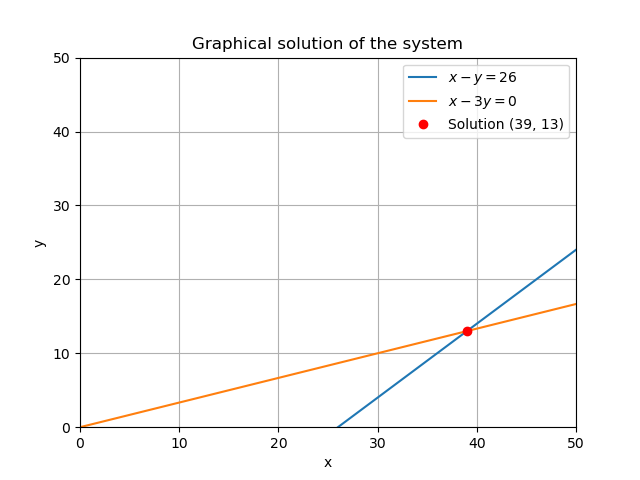
\includegraphics[width=\columnwidth, height=0.8\textheight, keepaspectratio]{Figs/Fig1.png}     
\end{frame}


\end{document}